\documentclass{ifacconf}
\usepackage[english]{babel}
\usepackage[T1]{fontenc}
\usepackage[utf8]{inputenc}
\usepackage{url}
\usepackage{graphicx}
\usepackage{natbib}
 
\bibpunct{(}{)}{;}{a}{,}{}

\usepackage{color}
\usepackage{subfig}

%nastavenie vypisov kodu
\usepackage{listings}
\usepackage{caption}

\captionsetup[lstlisting]{singlelinecheck=false}

\lstnewenvironment{code}[1][]%
  {\minipage{\columnwidth} 
   \lstset{
language=Python, 
basicstyle=\footnotesize,
numbers=left,
numberstyle=\tiny,
xleftmargin= 12pt,
abovecaptionskip=10pt,
stepnumber=1,
numbersep=5pt,
frame=none,
tabsize=2,
captionpos=b,
breaklines=true,
breakatwhitespace=false,
escapeinside={\%}{)}
}
}
  {\endminipage}

\lstset{
language=Python, 
basicstyle=\footnotesize,
numbers=left,
numberstyle=\tiny,
xleftmargin= 12pt,
abovecaptionskip=10pt,
stepnumber=1,
numbersep=5pt,
frame=none,
tabsize=2,
captionpos=b,
breaklines=true,
breakatwhitespace=false,
escapeinside={\%}{)}
}


\begin{document}
\begin{frontmatter}
\title{Simulation of 2D physics of objects captured by web camera using OpenCV
and Box2D}
\author[Bratislava]{Michal Sedlák}
\address[Bratislava]{Faculty of Electrical Engineering and Information
Technology, Slovak University of Technology, Ilkovičova 3, 812 19 Bratislava,
Slovakia
\\
(e-mail: michal.sedlak@stuba.sk)}
\begin{abstract}
The paper presents one approach to simulation of physics applied on objects
captured by web camera. Introduced approach utilise OpenCV library for image
capturing and contour detection. Objects detected by OpenCV are reconstructed
from its outlines in Box2D environment so the physics can be applied to it.
Because of restrictions of Box2D we needed to do approximation and scaling of
outlines and tessellation of objects with Delaunay triangulation algorithm.
\end{abstract}
\begin{keyword}
OpenCV, Python, Box2D, physics, tessellation
\end{keyword}
\end{frontmatter}

\section{Introduction}
This paper describes applying of Newtonian physics to hand drawn objects
recognized in image from camera. Simulation of physics is used in many modern
applications. You can find in implementations used by 3D drawing and animation
programs, more complex used in game engines or exact and precise simulation in
CAE programs. Paper describes process of animation of hand drawn object, from a
capturing phase, over recognition of the objects, interpretation objects in
physical engine, to animation of such objects. This approach can be applied in
education of physics at elementary schools, with interactive blackboards, or in
computer games.

\section{Object detection and Open Computer Vision library}
To apply a physics to hand drawn objects we need to identify and isolate
objects from image. We have used a web camera as a source and Open Computer
Vision library as processing tool of the images.

\subsection{OpenCV}
In regards the book of \cite{OpenCV} OpenCV  is a library for open source
programming functions for real time computer vision, with more than five hundred
optimized algorithms. It can be used with C++, C and Python. We chose Python for
implementation in our application.

Simple image capture is shown in Listing~\ref{Capture}.
\begin{lstlisting}[caption=Query image frame from web camera, label=Capture]
self.camera = cv.CaptureFromCAM(-1) %\label{Capture:init})
self.image = cv.QueryFrame(self.camera) %\label{Capture:query})
self.DetectOutline(self.image)
\end{lstlisting}
In line \ref{Capture:init} of Listing~\ref{Capture} we initialize our web
camera. In variable camera is allocated and initialized object that can query
camera for new image. Then as we see in \ref{Capture:query} we can get the
image from camera and store it in the variable named image. Captured image
is shown in Figure \ref{fig:captured}.
\begin{figure}[h]
\center
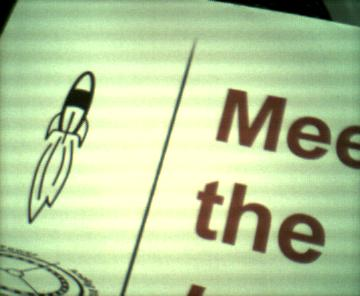
\includegraphics[width=0.8\columnwidth]{images/1test.png}
\caption{Image captured form camera}
\label{fig:captured}
\end{figure}

Now when we have image data stored in the variable, we can process data to find
outlines.

\begin{lstlisting}[caption=Outline detection, label=Detect]
def DetectOutline(self, image):
  image_size = cv.GetSize(image)
  grayscale = cv.CreateImage(image_size, 8, 1)	%\label{Detect:grayscale})
  cv.CvtColor(image, grayscale, cv.CV_BGR2GRAY)
  cv.EqualizeHist(grayscale, grayscale)	%\label{Detect:equalize})
  storage = cv.CreateMemStorage(0)
  cv.Threshold(grayscale, grayscale, 50, 255, cv.CV_THRESH_BINARY) %\label{Detect:threshold})
  self.contours = cv.FindContours(grayscale, %\label{Detect:contours})
    cv.CreateMemStorage(),
    cv.CV_RETR_TREE,
    cv.CV_CHAIN_APPROX_SIMPLE)
  if len(self.contours) > 0:
    self.contours = cv.ApproxPoly (self.contours, %\label{Detect:approx})
      storage,
      cv.CV_POLY_APPROX_DP,
      1.5,
      1)
  return self.contours
\end{lstlisting}

In function in Listing~\ref{Detect} is shown how to find outlines of objects in
image. We convert image to grey scale as seen on line \ref{Detect:grayscale}.

Then we run histogram equalization (line:~\ref{Detect:equalize}). Equalization
makes objects better visible and gives better output for thresholding
(line:~\ref{Detect:threshold}) which makes black and with image prepared for
outline detection (line:~\ref{Detect:contours}). Output of thresholding is
shown in (Figure \ref{fig:threshold}).

\begin{figure}[h]
  \center
  \subfloat[Equalize histogram]{
    \label{fig:histogram}
    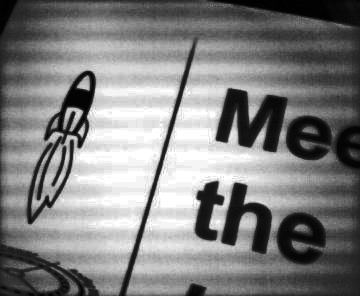
\includegraphics[width=0.48\columnwidth]{images/3test-equalize-histogram.png}
  }
  \subfloat[Thresholding]{
    \label{fig:threshold}
    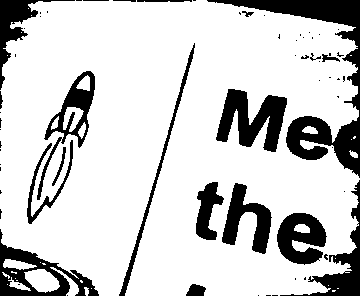
\includegraphics[width=0.48\columnwidth]{images/4test-threshold.png}
   }
\caption{Effects applied on images}
\label{fig:operations}
\end{figure}

After outline detection we have tree of contours stored in the variable
self.contours. These trees are iterable objects sorted from outer to inner
outline connected by property h\_next and v\_next that we will describe in
paragraph about creation of objects from outlines.

Contour can be very complicated and consist of thousands of points, which could
cause too complicated objects. It is time demanding to simulate complicated
objects, that is why we use polynomial approximation of the contour points.
(line:~\ref{Detect:approx}). Visualisation of outlines is shown in Figure:
\ref{fig:contours}.

\begin{figure}[h]
\center
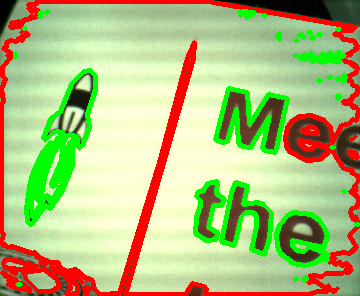
\includegraphics[width=0.8\columnwidth]{images/5test-contours.png}
\caption{Visualisation of contours}
\label{fig:contours}
\end{figure}

Now we have all outlines stored in the outline tree structure, so we can create
objects and apply a physics.

\section{Physics simulation in Box2D}
There is lot of physics engines that can be used for simulation of physics.
Because we wanted to simulate physics only in 2D we could, code our own
implementation of physics, or use one of commercial or open source engines. We
chose Box2D[\cite{GameEngines}], which is open source 2D physics engine with
possibility to simulate rigid body objects and their collisions.
\subsection{World}
To create physics simulation we need to create world. World is object that
manages memory, objects and simulation. Creation of world is shown in Listing
\ref{World}:
\begin{lstlisting}[caption=Creation of Box2D world,label=World]
self.worldAABB=box2d.b2AABB()
self.worldAABB.lowerBound = (-100.0, -100.0) %\label{World:lower})
self.worldAABB.upperBound = ( 600.0, 600.0)	%\label{World:upper})
gravity = (0.0, -10.0) %\label{World:gravity})

doSleep = True %\label{World:sleep})
self.world = box2d.b2World(self.worldAABB, gravity, doSleep)
\end{lstlisting}
First we have to create boundaries of the world. We define them as vectors from
bottom left (line:~\ref{World:lower}) to top right (line:~
\ref{World:upper}). Objects have to be inside the boundaries, when an object
touch the boundary it gets stuck. Then we define gravity vector (line:~
\ref{World:gravity}). The last thing before creation of the world we allow
objects to sleep(line:~\ref{World:sleep}). Object that are not moving fall
asleep, then are ignored by the engine. Last line of Listing~\ref{World} creates
the world.

World is created and we are ready to create objects from outlines.
\subsection{Objects}
Every object that is simulated in Box2D consists of body and shapes. Our objects
are described by the contour tree. To create objects we need to iterate contour
tree, find contours that belongs to together and create objects for these
contours.
\subsection{Contour tree}
Contour tree is object in which are stored points of each contour. Contours are
connected by functions returning reference to other contours with h\_next() and
v\_next(). h\_next() is referencing to deeper contour, and v\_next is
referencing to another object contour. To iterate over all contours we have
created recursive function shown in Listing: \ref{CreateObjects}.
\begin{lstlisting}[label=CreateObjects,caption=Function to iterate through
contour tree]
def CreateObjectsFromCountours(self, cont, h=0, v=0):
  if v>0:	%\label{CreateObjects:depth})
    density = 10.0 %\label{CreateObjects:density10})
  else:
    density = 0 %\label{CreateObjects:density0})
  if len(cont)>8:
    self.CreateObject(cont,h,v) 

  if cont.v_next():
    v += 1
    self.CreateObjectsFromCountours(cont.v_next(),h,v)
    v -= 1

  if cont.h_next():
    h += 1
    self.CreateObjectsFromCountours(cont.h_next(),h,v)
\end{lstlisting}
We iterate through contour tree. First level is outer contour of the image
(line:~\ref{CreateObjects:depth}), because we do not want the outer contour to
move, we set it as static by setting density to 0 (line:~
\ref{CreateObjects:density0}). Every other contour is dynamic body with density
set to 10 (line:~\ref{CreateObjects:density10}).

When we know what type of object we will create, we can create bodies and
shapes for our contours.
\subsection{Bodies, shapes and collisions}
Bodies are backbone used by shapes. One body can contain more shapes, but one
shape could be attached to only one body. Box2d is rigid body physics engine,
that mean that shapes attached to body can not move against other, or body. Body
have position and velocity. Forces, torques and impulses can be applied to body
[\cite{Box2DManual}].  Bodies just hold the shapes. Shapes are elements that
collide together.

Listings \ref{Objects1},\ref{Objects2},\ref{Objects3} shows how to create object
from outer contour:
\begin{lstlisting}[name=Objects,label=Objects1,caption=Creation of object from
outer contour]
def CreateObject(self, cont, h,v):
  contM = []
  for point in cont:
    x = point[0]/30.0	%\label{Objects:scaling})
    y = point[1]/30.0
    contM.append((x,y))
    
  bd=box2d.b2BodyDef() %\label{Objects:CreateBody})
  bd.position = ( 0.0, 0.0 )
  
  edgeDef=box2d.b2EdgeChainDef() %\label{Objects:CreateChain})
  edgeDef.setVertices(contM) %\label{Objects:AssignVertices})

  if v==0:
    body = self.world.CreateBody(bd)
    try:
      self.contourBodies.append(body)
    except:
      self.contourBodies = [body] %\label{Objects:CountourBodies})
      body.CreateShape(edgeDef) %\label{Objects:AttachShape})
\end{lstlisting}
Image size is measured in pixels and Box2D units are kilograms, meters,
and seconds (KMS) we should scale images coordinates to fit in 0.1m to
10m. In that scale is performance of Box2D the best. We are doing it by
dividing of value of pixel coordinates by 30.0 (line:~\ref{Objects:scaling})

Then we create a body definition that will represent our contour(line:~
\ref{Objects:CreateBody}) and set up it initial position in next line.

After that we create shape of body as chain of edges (line:~
\ref{Objects:CreateChain}) and assign the array of vertices to it (line:~
\ref{Objects:AssignVertices}). Edges are special type of shapes that have no
mass, is represented as line between vertices that collide with other non-edge
objects. Edges are easy to create because they do not have to be concave unlike
polygons.

At last we attach this shape to created body \ref{Objects:AttachShape}. Because
Box2D does not keep track about body definitions, we have to store bodies in to
array for later use (line: \ref{Objects:CountourBodies}).

Listing of the function CreateObject() continuous in Listing~\ref{Objects2}. This
part of function creates dynamic objects inside the outer contour. In this part
we prepare list for bodies of objects, so we can modify objects that are already
created or objects that we want append new shapes.
\begin{lstlisting}[name=Objects,firstnumber=auto,label=Objects2,caption=Creation of objects] if v == 1:
    try:
      body = self.objectBodies[h]
    except:
      body = self.world.CreateBody(bd)
      self.objectBodies[h] = body
\end{lstlisting}
\subsection{tessellation}
Box2D supports only collisions between convex objects and contours of objects
captured by camera are not convex we have to break outlines to convex polygons.
There is more ways how to break concave objects. We chose the 2D constrained
Delaunay triangulation algorithm implemented by poly2tri Python
library[\cite{Delauanay}]. Function CreateObject() continuous in Listing~
\ref{Objects3}
\begin{lstlisting}[name=Objects,firstnumber=auto,label=Objects3,caption=Creation
 of objects]
    polyline = []
    for (x,y) in cont:
      polyline.append(p2t.Point(x,y)) %\label{Objects:polyline})
    cdt = p2t.CDT(polyline) %\label{Objects:p2t})
    triangles = cdt.triangulate()
    for t in triangles:  %\label{Objects:scale1})
      x1 = t.a.x/30.0
      y1 = t.a.y/30.0
      x2 = t.b.x/30.0
      y2 = t.b.y/30.0
      x3 = t.c.x/30.0
      y3 = t.c.y/30.0  %\label{Objects:scale2})
      if math.hypot(x2-x1,y2-y1)<0.1: %\label{Objects:minSize1})
        x2 = x2 + math.copysign(0.1, x2-x1)
        y2 = y2 + math.copysign(0.1, y2-y1)
      if math.hypot(x3-x2,y3-y2)<0.1:
        x3 = x3 + math.copysign(0.1, x3-x2)
        y3 = y3 + math.copysign(0.1, y3-y2)
      if math.hypot(x1-x3,y1-y3)<0.1:
        x1 = x1 + math.copysign(0.1, x1-x3)
        y1 = y1 + math.copysign(0.1, y1-y3) %\label{Objects:minSize2})
      poly=box2d.b2PolygonDef()  %\label{Objects:polygondef})
      poly.setVertices(((x1, y1), (x2, y2), (x3, y3)))
      poly.density = 1.0
      poly.restitution = 0.0
      poly.friction = 0.0
      body.CreateShape(poly)  %\label{Objects:createshape})
      body.SetMassFromShapes() %\label{Objects:setMass})
\end{lstlisting}
The creation of objects continues with tessellation. We need to assign vertices
to structure that could be understood by poly2tri library
(line:~\ref{Objects:polyline}) and we initialize the CDT object
(line:~\ref{Objects:p2t}). In next line we call function that will create
triangles from the vertices assigned before. These triangles are in image pixel
coordinates, so we need to scale them at first
(lines:~\ref{Objects:scale1}-\ref{Objects:scale2}). Now when we have triangles
scaled we need to scale the triangles that are too small to triangles with size
at least 0.1m because of speed optimalization, this is done in
lines:~\ref{Objects:minSize1}-\ref{Objects:minSize2}). Now we have set of
triangular shapes that could be attached to body
(line:~\ref{Objects:createshape:}). Because these objects are compound objects,
we need to set the center of mass and amount to this body. We can let Box2D set
this properties based on shape information with body function
SetMassFromShapes() (line:~\ref{Objects:setMass}). Visualisation of objects is
in Figure \ref{fig:objects}.

\begin{figure}[h]
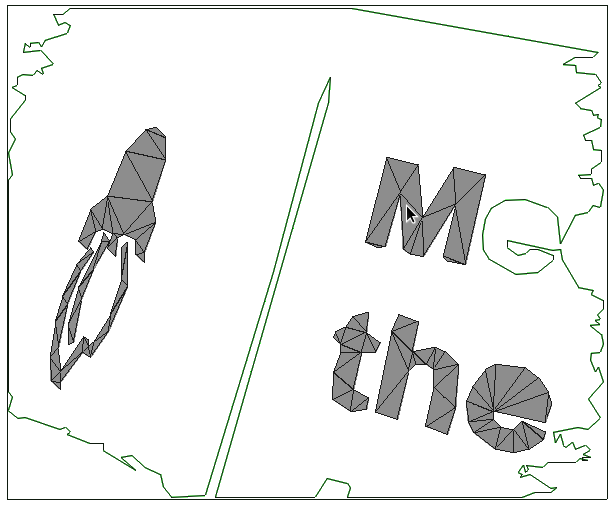
\includegraphics[width=\columnwidth]{images/6dynamic-objets.png}
\caption{Visualisation of objects after triangulation}
\label{fig:objects}
\end{figure}

After this we can add other objects and start simulation by function \lstinline{Step()}.
After few second of simulation are all objects on the bottom of the screen like
is shown in figure \ref{fig:simulation}.

\begin{figure}[h]
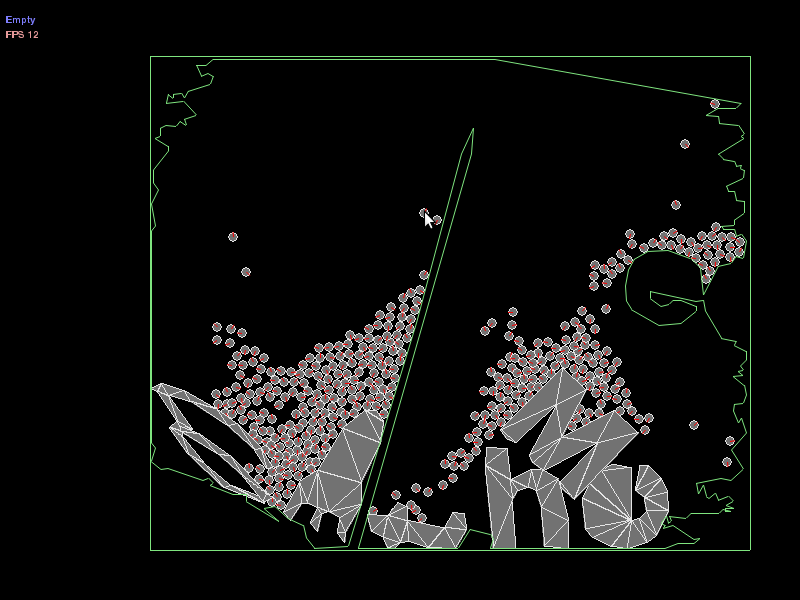
\includegraphics[width=\columnwidth]{images/7dynamic-objets-simulation.png}
\caption{Visualisation of simulation}
\label{fig:simulation}
\end{figure}

\section{Future work}
This approach can be used in interactive blackboards used for education of
physics on elementary schools, in future work we plan to implement
identification of some special objects like springs or joints.

We are planning to implement object tracking, and dynamic object morphing so we
could interact with simulated objects. Because of Box2D is rigid body engine,
is complicated to simulate physics of objects that change their shape in time.
We plan to implement some soft body elements to make this possible.

The last stage will be usage of captured images as source of textures of
simulated objects. Because this is only decorative element, we are planning to
implement this task as a last one.

\section*{Acknowledgments}
The work was supported by a grant (No. NIL-I-007-d) from Iceland, Liechtenstein 
and Norway through the EEA Financial Mechanism and the Norwegian Financial 
Mechanism. This project is also co-financed from the state budget of the Slovak
Republic.

%If you use BibTeX comment the second line, if not comment the first line
\bibliography{pcbib}
%\documentclass{ifacconf}
\usepackage[english]{babel}
\usepackage[T1]{fontenc}
\usepackage[utf8]{inputenc}
\usepackage{natbib}

\bibpunct{(}{)}{;}{a}{,}{}

\usepackage{color}
\usepackage{listings}
\lstset{ %
language=Python, 
basicstyle=\footnotesize,
numbers=left,
numberstyle=\tiny,
xleftmargin= 10pt,
stepnumber=1,
numbersep=5pt,
backgroundcolor=\color{white}, 
showspaces=false,
showstringspaces=false,
showtabs=false,
frame=none,
tabsize=2,
captionpos=b,
breaklines=true,
breakatwhitespace=false,
escapeinside={\%}{)}
}

\begin{document}
\begin{frontmatter}
\title{Simulation of 2D physics of hand drawn objects using OpenCV and Box2D}
\author[Bratislava]{Michal Sedlák}
\address[Bratislava]{Faculty of Electrical Engineering and Information
Technology, Slovak University of Technology, Ilkovičova 3, 812 19 Bratislava,
Slovakia
\\
(e-mail: michal.sedlak@stuba.sk)}
\begin{abstract}
%TODO Napisat abstrakt

\end{abstract}
\begin{keyword}
Maximum 5 keywords.
\end{keyword}
\end{frontmatter}

\section{Introduction}
This paper describes applying of Newtonian physics to hand drawn objects
recognized in image from camera. Simulation of physics is used in many modern
applications. You can find in implementations used by 3D drawing and animation
programs, more complex used in game engines or exact and precise simulation in
CAE programs. Paper describes process of animation of hand drawn object, from a
capturing phase, over recognition of the objects, interpretation objects in
physical engine, to animation of such objects. This approach can be applied in
education of physics at elementary schools, with interactive blackboards, or in
computer games.

\section{Object detection and Open Computer Vision library}
To apply a physics to hand drawn objects we need to identify and isolate
objects from image. We have used a web camera as a source and Open Computer
Vision library as processing tool of the images.

\subsection{OpenCV}
In regards the book of \cite{OpenCV} OpenCV  is a library for open source
programming functions for real time computer vision, with more than five hundred
optimized algorithms. It can be used with C++, C and Python. We chose Python for
implementation in our application.

Simple image capture is shown in Listing \ref{Capture}.
\begin{lstlisting}[caption=Query image frame from web camera, label=Capture]
self.camera = cv.CaptureFromCAM(-1) %\label{Capture:init})
self.image = cv.QueryFrame(self.camera) %\label{Capture:query})
self.DetectOutline(self.image)
\end{lstlisting}
In line \ref{Capture:init} of listing \ref{Capture} we initialize our web
camera. In variable camera is allocated and initialized object that can query
camera for new image. Then as we see in \ref{Capture:query} we can get the
image from camera and store it in the variable named image. Now when we have
image data stored in the variable, we can process data to find outlines.
\begin{lstlisting}[caption=Outline detection, label=Detect]
def DetectOutline(self, image):
  image_size = cv.GetSize(image)
  grayscale = cv.CreateImage(image_size, 8, 1)	%\label{Detect:grayscale})
  cv.CvtColor(image, grayscale, cv.CV_BGR2GRAY)
  cv.EqualizeHist(grayscale, grayscale)	%\label{Detect:equalize})
  storage = cv.CreateMemStorage(0)
  cv.Threshold(grayscale, grayscale, 50, 255, cv.CV_THRESH_BINARY) %\label{Detect:threshold})
  self.contours = cv.FindContours(grayscale, %\label{Detect:contours})
    cv.CreateMemStorage(),
    cv.CV_RETR_TREE,
    cv.CV_CHAIN_APPROX_SIMPLE)
  if len(self.contours) > 0:
    self.contours = cv.ApproxPoly (self.contours, %\label{Detect:approx})
      storage,
      cv.CV_POLY_APPROX_DP,
      1.5,
      1)
  return self.contours
\end{lstlisting}
In function in Listing \ref{Detect} is shown how to find outlines of objects in
image. We convert image to gray scale as seen on line \ref{Detect:grayscale}.
Then we run histogram equalization (line: \ref{Detect:equalize}).
Equalization makes objects better visible and gives better output for
thresholding (line: \ref{Detect:threshold}) which makes black and white image
prepared for outline detection (line: \ref{Detect:contours}).
%TODO Doplnit obrazok s normalizaciou histogramu
%TODO Doplnit obrazok s thresholdom
After outline detection we have tree of contours stored in the variable
self.contours. These trees are iterable objects sorted from outer to inner
outline connected by property h\_next and v\_next that we will describe in
paragraph about creation of objects from outlines.

Contour can be very complicated and consist of thousands of points, which could
cause too complicated objects. It is time demanding to simulate complicated
objects, that is why we use polynomial approximation of the contour points.
(line:~\ref{Detect:approx}).

Now we have all outlines stored in the outline tree structure, so we can create
objects and apply a physics.
%TODO Doplnit obrazok so zvyraznenymi outlineami

\section{Physics simulation in Box2D}
There is lot of physics engines that can be used for simulation of physics.
Because we wanted to simulate physics only in 2D we could, code our own
implementation of physics, or use one of commercial or open source engines. We
chose Box2D[\cite{GameEngines}], which is open source 2D physiscs engine with
posibility to simulate rigid body objects and their collisions.
\subsection{World}
To create physics simulation we need to create world. World is object that
manages memory, objects and simulation. Creation of world is shown in Listing
\ref{World}:
\begin{lstlisting}[caption=Creation of Box2D world,label=World]
self.worldAABB=box2d.b2AABB()
self.worldAABB.lowerBound = (-100.0, -100.0) %\label{World:lower})
self.worldAABB.upperBound = ( 600.0, 600.0)	%\label{World:upper})
gravity = (0.0, -10.0) %\label{World:gravity})

doSleep = True %\label{World:sleep})
self.world = box2d.b2World(self.worldAABB, gravity, doSleep)
\end{lstlisting}
First we have to create boundaries of the world. We define them as vectors from
bottom left (line: \ref{World:lower}) to top right (line:
\ref{World:upper}). Objects have to be inside the boudaries, when an object
touch the boundary it gets stuck. Then we define gravity vector (line:
\ref{World:gravity}). The last thing before creation of the world we allow
objects to sleep(line: \ref{World:sleep}). Object that are not moving fall
asleep, then are ignored by the engine. Last line of Listing \ref{World} creates
the world.

When we have world created we are ready to create objects from outlines.
\subsection{Objects}
Every object that is simulated in Box2D consists of body and shapes.
\subsubsection{Bodies, shapes and collisions}
Bodies are skelet used by shapes. One body can contain more shapes, but one
shape could be attached to only one body. Box2d is rigid body
physics engine, that mean that shapes attached to body can not move against
other, or body.
\subsection{Tesselation}
Box2D supports only collisions between convex objects. That is why we need to
breake outlines to convex polygons. There is more ways how to break concave
objects. We chose Seidel's Triangulation Algorithm implemented by poly2tri
Python library
%TODO asi iny algorytmus
%TODO pridat referenciu na poly2tri

\subsection{Implementation}
%TODO dat sem zdrojovy kod a popisat ho
\section{Future work}
Identifikacia objektov
Sledovanie objektov a morfing
Interakcia hybucich sa objektov zachytenych kamerov s Box2D reprezentaciou

\section*{Acknowledgments}
The work was supported by a grant (No. NIL-I-007-d) from Iceland, Liechtenstein 
and Norway through the EEA Financial Mechanism and the Norwegian Financial 
Mechanism. This project is also co-financed from the state budget of the Slovak
Republic..

%If you use BibTeX comment the second line, if not comment the first line
\bibliography{pcbib}
%\documentclass{ifacconf}
\usepackage[english]{babel}
\usepackage[T1]{fontenc}
\usepackage[utf8]{inputenc}
\usepackage{natbib}

\bibpunct{(}{)}{;}{a}{,}{}

\usepackage{color}
\usepackage{listings}
\lstset{ %
language=Python, 
basicstyle=\footnotesize,
numbers=left,
numberstyle=\tiny,
xleftmargin= 10pt,
stepnumber=1,
numbersep=5pt,
backgroundcolor=\color{white}, 
showspaces=false,
showstringspaces=false,
showtabs=false,
frame=none,
tabsize=2,
captionpos=b,
breaklines=true,
breakatwhitespace=false,
escapeinside={\%}{)}
}

\begin{document}
\begin{frontmatter}
\title{Simulation of 2D physics of hand drawn objects using OpenCV and Box2D}
\author[Bratislava]{Michal Sedlák}
\address[Bratislava]{Faculty of Electrical Engineering and Information
Technology, Slovak University of Technology, Ilkovičova 3, 812 19 Bratislava,
Slovakia
\\
(e-mail: michal.sedlak@stuba.sk)}
\begin{abstract}
%TODO Napisat abstrakt

\end{abstract}
\begin{keyword}
Maximum 5 keywords.
\end{keyword}
\end{frontmatter}

\section{Introduction}
This paper describes applying of Newtonian physics to hand drawn objects
recognized in image from camera. Simulation of physics is used in many modern
applications. You can find in implementations used by 3D drawing and animation
programs, more complex used in game engines or exact and precise simulation in
CAE programs. Paper describes process of animation of hand drawn object, from a
capturing phase, over recognition of the objects, interpretation objects in
physical engine, to animation of such objects. This approach can be applied in
education of physics at elementary schools, with interactive blackboards, or in
computer games.

\section{Object detection and Open Computer Vision library}
To apply a physics to hand drawn objects we need to identify and isolate
objects from image. We have used a web camera as a source and Open Computer
Vision library as processing tool of the images.

\subsection{OpenCV}
In regards the book of \cite{OpenCV} OpenCV  is a library for open source
programming functions for real time computer vision, with more than five hundred
optimized algorithms. It can be used with C++, C and Python. We chose Python for
implementation in our application.

Simple image capture is shown in Listing \ref{Capture}.
\begin{lstlisting}[caption=Query image frame from web camera, label=Capture]
self.camera = cv.CaptureFromCAM(-1) %\label{Capture:init})
self.image = cv.QueryFrame(self.camera) %\label{Capture:query})
self.DetectOutline(self.image)
\end{lstlisting}
In line \ref{Capture:init} of listing \ref{Capture} we initialize our web
camera. In variable camera is allocated and initialized object that can query
camera for new image. Then as we see in \ref{Capture:query} we can get the
image from camera and store it in the variable named image. Now when we have
image data stored in the variable, we can process data to find outlines.
\begin{lstlisting}[caption=Outline detection, label=Detect]
def DetectOutline(self, image):
  image_size = cv.GetSize(image)
  grayscale = cv.CreateImage(image_size, 8, 1)	%\label{Detect:grayscale})
  cv.CvtColor(image, grayscale, cv.CV_BGR2GRAY)
  cv.EqualizeHist(grayscale, grayscale)	%\label{Detect:equalize})
  storage = cv.CreateMemStorage(0)
  cv.Threshold(grayscale, grayscale, 50, 255, cv.CV_THRESH_BINARY) %\label{Detect:threshold})
  self.contours = cv.FindContours(grayscale, %\label{Detect:contours})
    cv.CreateMemStorage(),
    cv.CV_RETR_TREE,
    cv.CV_CHAIN_APPROX_SIMPLE)
  if len(self.contours) > 0:
    self.contours = cv.ApproxPoly (self.contours, %\label{Detect:approx})
      storage,
      cv.CV_POLY_APPROX_DP,
      1.5,
      1)
  return self.contours
\end{lstlisting}
In function in Listing \ref{Detect} is shown how to find outlines of objects in
image. We convert image to gray scale as seen on line \ref{Detect:grayscale}.
Then we run histogram equalization (line: \ref{Detect:equalize}).
Equalization makes objects better visible and gives better output for
thresholding (line: \ref{Detect:threshold}) which makes black and white image
prepared for outline detection (line: \ref{Detect:contours}).
%TODO Doplnit obrazok s normalizaciou histogramu
%TODO Doplnit obrazok s thresholdom
After outline detection we have tree of contours stored in the variable
self.contours. These trees are iterable objects sorted from outer to inner
outline connected by property h\_next and v\_next that we will describe in
paragraph about creation of objects from outlines.

Contour can be very complicated and consist of thousands of points, which could
cause too complicated objects. It is time demanding to simulate complicated
objects, that is why we use polynomial approximation of the contour points.
(line:~\ref{Detect:approx}).

Now we have all outlines stored in the outline tree structure, so we can create
objects and apply a physics.
%TODO Doplnit obrazok so zvyraznenymi outlineami

\section{Physics simulation in Box2D}
There is lot of physics engines that can be used for simulation of physics.
Because we wanted to simulate physics only in 2D we could, code our own
implementation of physics, or use one of commercial or open source engines. We
chose Box2D[\cite{GameEngines}], which is open source 2D physiscs engine with
posibility to simulate rigid body objects and their collisions.
\subsection{World}
To create physics simulation we need to create world. World is object that
manages memory, objects and simulation. Creation of world is shown in Listing
\ref{World}:
\begin{lstlisting}[caption=Creation of Box2D world,label=World]
self.worldAABB=box2d.b2AABB()
self.worldAABB.lowerBound = (-100.0, -100.0) %\label{World:lower})
self.worldAABB.upperBound = ( 600.0, 600.0)	%\label{World:upper})
gravity = (0.0, -10.0) %\label{World:gravity})

doSleep = True %\label{World:sleep})
self.world = box2d.b2World(self.worldAABB, gravity, doSleep)
\end{lstlisting}
First we have to create boundaries of the world. We define them as vectors from
bottom left (line: \ref{World:lower}) to top right (line:
\ref{World:upper}). Objects have to be inside the boudaries, when an object
touch the boundary it gets stuck. Then we define gravity vector (line:
\ref{World:gravity}). The last thing before creation of the world we allow
objects to sleep(line: \ref{World:sleep}). Object that are not moving fall
asleep, then are ignored by the engine. Last line of Listing \ref{World} creates
the world.

When we have world created we are ready to create objects from outlines.
\subsection{Objects}
Every object that is simulated in Box2D consists of body and shapes.
\subsubsection{Bodies, shapes and collisions}
Bodies are skelet used by shapes. One body can contain more shapes, but one
shape could be attached to only one body. Box2d is rigid body
physics engine, that mean that shapes attached to body can not move against
other, or body.
\subsection{Tesselation}
Box2D supports only collisions between convex objects. That is why we need to
breake outlines to convex polygons. There is more ways how to break concave
objects. We chose Seidel's Triangulation Algorithm implemented by poly2tri
Python library
%TODO asi iny algorytmus
%TODO pridat referenciu na poly2tri

\subsection{Implementation}
%TODO dat sem zdrojovy kod a popisat ho
\section{Future work}
Identifikacia objektov
Sledovanie objektov a morfing
Interakcia hybucich sa objektov zachytenych kamerov s Box2D reprezentaciou

\section*{Acknowledgments}
The work was supported by a grant (No. NIL-I-007-d) from Iceland, Liechtenstein 
and Norway through the EEA Financial Mechanism and the Norwegian Financial 
Mechanism. This project is also co-financed from the state budget of the Slovak
Republic..

%If you use BibTeX comment the second line, if not comment the first line
\bibliography{pcbib}
%\documentclass{ifacconf}
\usepackage[english]{babel}
\usepackage[T1]{fontenc}
\usepackage[utf8]{inputenc}
\usepackage{natbib}

\bibpunct{(}{)}{;}{a}{,}{}

\usepackage{color}
\usepackage{listings}
\lstset{ %
language=Python, 
basicstyle=\footnotesize,
numbers=left,
numberstyle=\tiny,
xleftmargin= 10pt,
stepnumber=1,
numbersep=5pt,
backgroundcolor=\color{white}, 
showspaces=false,
showstringspaces=false,
showtabs=false,
frame=none,
tabsize=2,
captionpos=b,
breaklines=true,
breakatwhitespace=false,
escapeinside={\%}{)}
}

\begin{document}
\begin{frontmatter}
\title{Simulation of 2D physics of hand drawn objects using OpenCV and Box2D}
\author[Bratislava]{Michal Sedlák}
\address[Bratislava]{Faculty of Electrical Engineering and Information
Technology, Slovak University of Technology, Ilkovičova 3, 812 19 Bratislava,
Slovakia
\\
(e-mail: michal.sedlak@stuba.sk)}
\begin{abstract}
%TODO Napisat abstrakt

\end{abstract}
\begin{keyword}
Maximum 5 keywords.
\end{keyword}
\end{frontmatter}

\section{Introduction}
This paper describes applying of Newtonian physics to hand drawn objects
recognized in image from camera. Simulation of physics is used in many modern
applications. You can find in implementations used by 3D drawing and animation
programs, more complex used in game engines or exact and precise simulation in
CAE programs. Paper describes process of animation of hand drawn object, from a
capturing phase, over recognition of the objects, interpretation objects in
physical engine, to animation of such objects. This approach can be applied in
education of physics at elementary schools, with interactive blackboards, or in
computer games.

\section{Object detection and Open Computer Vision library}
To apply a physics to hand drawn objects we need to identify and isolate
objects from image. We have used a web camera as a source and Open Computer
Vision library as processing tool of the images.

\subsection{OpenCV}
In regards the book of \cite{OpenCV} OpenCV  is a library for open source
programming functions for real time computer vision, with more than five hundred
optimized algorithms. It can be used with C++, C and Python. We chose Python for
implementation in our application.

Simple image capture is shown in Listing \ref{Capture}.
\begin{lstlisting}[caption=Query image frame from web camera, label=Capture]
self.camera = cv.CaptureFromCAM(-1) %\label{Capture:init})
self.image = cv.QueryFrame(self.camera) %\label{Capture:query})
self.DetectOutline(self.image)
\end{lstlisting}
In line \ref{Capture:init} of listing \ref{Capture} we initialize our web
camera. In variable camera is allocated and initialized object that can query
camera for new image. Then as we see in \ref{Capture:query} we can get the
image from camera and store it in the variable named image. Now when we have
image data stored in the variable, we can process data to find outlines.
\begin{lstlisting}[caption=Outline detection, label=Detect]
def DetectOutline(self, image):
  image_size = cv.GetSize(image)
  grayscale = cv.CreateImage(image_size, 8, 1)	%\label{Detect:grayscale})
  cv.CvtColor(image, grayscale, cv.CV_BGR2GRAY)
  cv.EqualizeHist(grayscale, grayscale)	%\label{Detect:equalize})
  storage = cv.CreateMemStorage(0)
  cv.Threshold(grayscale, grayscale, 50, 255, cv.CV_THRESH_BINARY) %\label{Detect:threshold})
  self.contours = cv.FindContours(grayscale, %\label{Detect:contours})
    cv.CreateMemStorage(),
    cv.CV_RETR_TREE,
    cv.CV_CHAIN_APPROX_SIMPLE)
  if len(self.contours) > 0:
    self.contours = cv.ApproxPoly (self.contours, %\label{Detect:approx})
      storage,
      cv.CV_POLY_APPROX_DP,
      1.5,
      1)
  return self.contours
\end{lstlisting}
In function in Listing \ref{Detect} is shown how to find outlines of objects in
image. We convert image to gray scale as seen on line \ref{Detect:grayscale}.
Then we run histogram equalization (line: \ref{Detect:equalize}).
Equalization makes objects better visible and gives better output for
thresholding (line: \ref{Detect:threshold}) which makes black and white image
prepared for outline detection (line: \ref{Detect:contours}).
%TODO Doplnit obrazok s normalizaciou histogramu
%TODO Doplnit obrazok s thresholdom
After outline detection we have tree of contours stored in the variable
self.contours. These trees are iterable objects sorted from outer to inner
outline connected by property h\_next and v\_next that we will describe in
paragraph about creation of objects from outlines.

Contour can be very complicated and consist of thousands of points, which could
cause too complicated objects. It is time demanding to simulate complicated
objects, that is why we use polynomial approximation of the contour points.
(line:~\ref{Detect:approx}).

Now we have all outlines stored in the outline tree structure, so we can create
objects and apply a physics.
%TODO Doplnit obrazok so zvyraznenymi outlineami

\section{Physics simulation in Box2D}
There is lot of physics engines that can be used for simulation of physics.
Because we wanted to simulate physics only in 2D we could, code our own
implementation of physics, or use one of commercial or open source engines. We
chose Box2D[\cite{GameEngines}], which is open source 2D physiscs engine with
posibility to simulate rigid body objects and their collisions.
\subsection{World}
To create physics simulation we need to create world. World is object that
manages memory, objects and simulation. Creation of world is shown in Listing
\ref{World}:
\begin{lstlisting}[caption=Creation of Box2D world,label=World]
self.worldAABB=box2d.b2AABB()
self.worldAABB.lowerBound = (-100.0, -100.0) %\label{World:lower})
self.worldAABB.upperBound = ( 600.0, 600.0)	%\label{World:upper})
gravity = (0.0, -10.0) %\label{World:gravity})

doSleep = True %\label{World:sleep})
self.world = box2d.b2World(self.worldAABB, gravity, doSleep)
\end{lstlisting}
First we have to create boundaries of the world. We define them as vectors from
bottom left (line: \ref{World:lower}) to top right (line:
\ref{World:upper}). Objects have to be inside the boudaries, when an object
touch the boundary it gets stuck. Then we define gravity vector (line:
\ref{World:gravity}). The last thing before creation of the world we allow
objects to sleep(line: \ref{World:sleep}). Object that are not moving fall
asleep, then are ignored by the engine. Last line of Listing \ref{World} creates
the world.

When we have world created we are ready to create objects from outlines.
\subsection{Objects}
Every object that is simulated in Box2D consists of body and shapes.
\subsubsection{Bodies, shapes and collisions}
Bodies are skelet used by shapes. One body can contain more shapes, but one
shape could be attached to only one body. Box2d is rigid body
physics engine, that mean that shapes attached to body can not move against
other, or body.
\subsection{Tesselation}
Box2D supports only collisions between convex objects. That is why we need to
breake outlines to convex polygons. There is more ways how to break concave
objects. We chose Seidel's Triangulation Algorithm implemented by poly2tri
Python library
%TODO asi iny algorytmus
%TODO pridat referenciu na poly2tri

\subsection{Implementation}
%TODO dat sem zdrojovy kod a popisat ho
\section{Future work}
Identifikacia objektov
Sledovanie objektov a morfing
Interakcia hybucich sa objektov zachytenych kamerov s Box2D reprezentaciou

\section*{Acknowledgments}
The work was supported by a grant (No. NIL-I-007-d) from Iceland, Liechtenstein 
and Norway through the EEA Financial Mechanism and the Norwegian Financial 
Mechanism. This project is also co-financed from the state budget of the Slovak
Republic..

%If you use BibTeX comment the second line, if not comment the first line
\bibliography{pcbib}
%\input{paper.bbl}

\end{document}





\end{document}





\end{document}





\end{document}
